\noindent
Dado que el objetivo del proyecto es comparar tres diferentes métodos 
de súper resolución, en esta sección se presentarán las actividades
requeridas para la implementación de los métodos. Considerando desde los 
requisitos de software, hardware y datos de entrenamiento en caso sean 
necesarios. 

\subsection{Example-Based Super-Resolution}
\subsubsection{Construcción de diccionario}
\noindent
Para el primero de ellos, se retoma la literatura expuesta en \cite{freeman}
comenzando con la generación del diccionario donde se encuentran relacionados 
los parches de baja y alta resolución. Previo a esto, es necesario pre-procesar
el conjunto de imágenes para su posterior segmentación. 

De acuerdo a las indicaciones, se deben tener pares de imágenes en alta y baja 
resolución. Para esta implementación se ha considerado las primeras 14 imágenes
de \cite{MIRFLICKR} las cuales están en alta resolución. En la Figura \ref{fig:fr_dataset}
puede observarse que el conjunto de imágenes no guardan una relación en específico
por lo que los requisitos para aplicar el algoritmo son bastante flexibles.

\begin{figure}[H]
    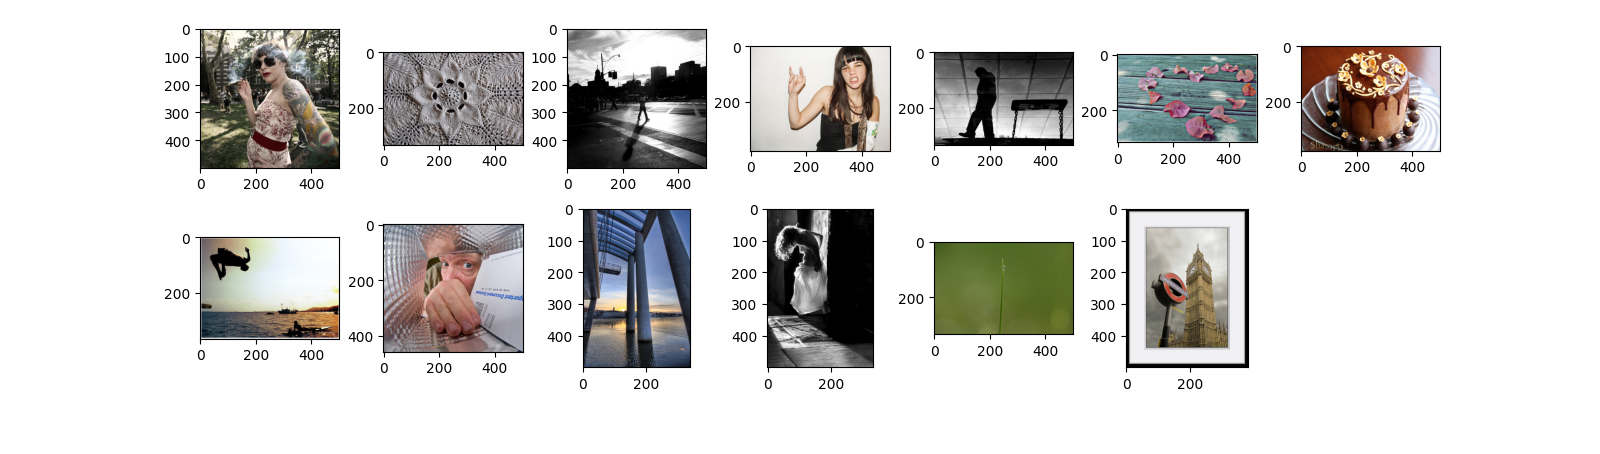
\includegraphics[scale = 0.4]{ fr_dataset.png }
    \centering
    \caption{ \emph{Dataset} utilizado para construcción de diccionario}
    \label{fig:fr_dataset}
\end{figure}

En la Figura \ref{fig:fr_interpolacion} se presenta el procedimiento realizado para
construir el conjunto de imágenes de baja resolución mediante una reducción por el 
factor $\frac{1}{\Omega}$ y posterior escalado de $\Omega$ con el objetivo de 
perder información al escalar la imagen una vez realizada la compresión, forzando
la baja resolución. Para esta implementación se consideró un factor $\Omega = 4$. 

\begin{figure}[H]
    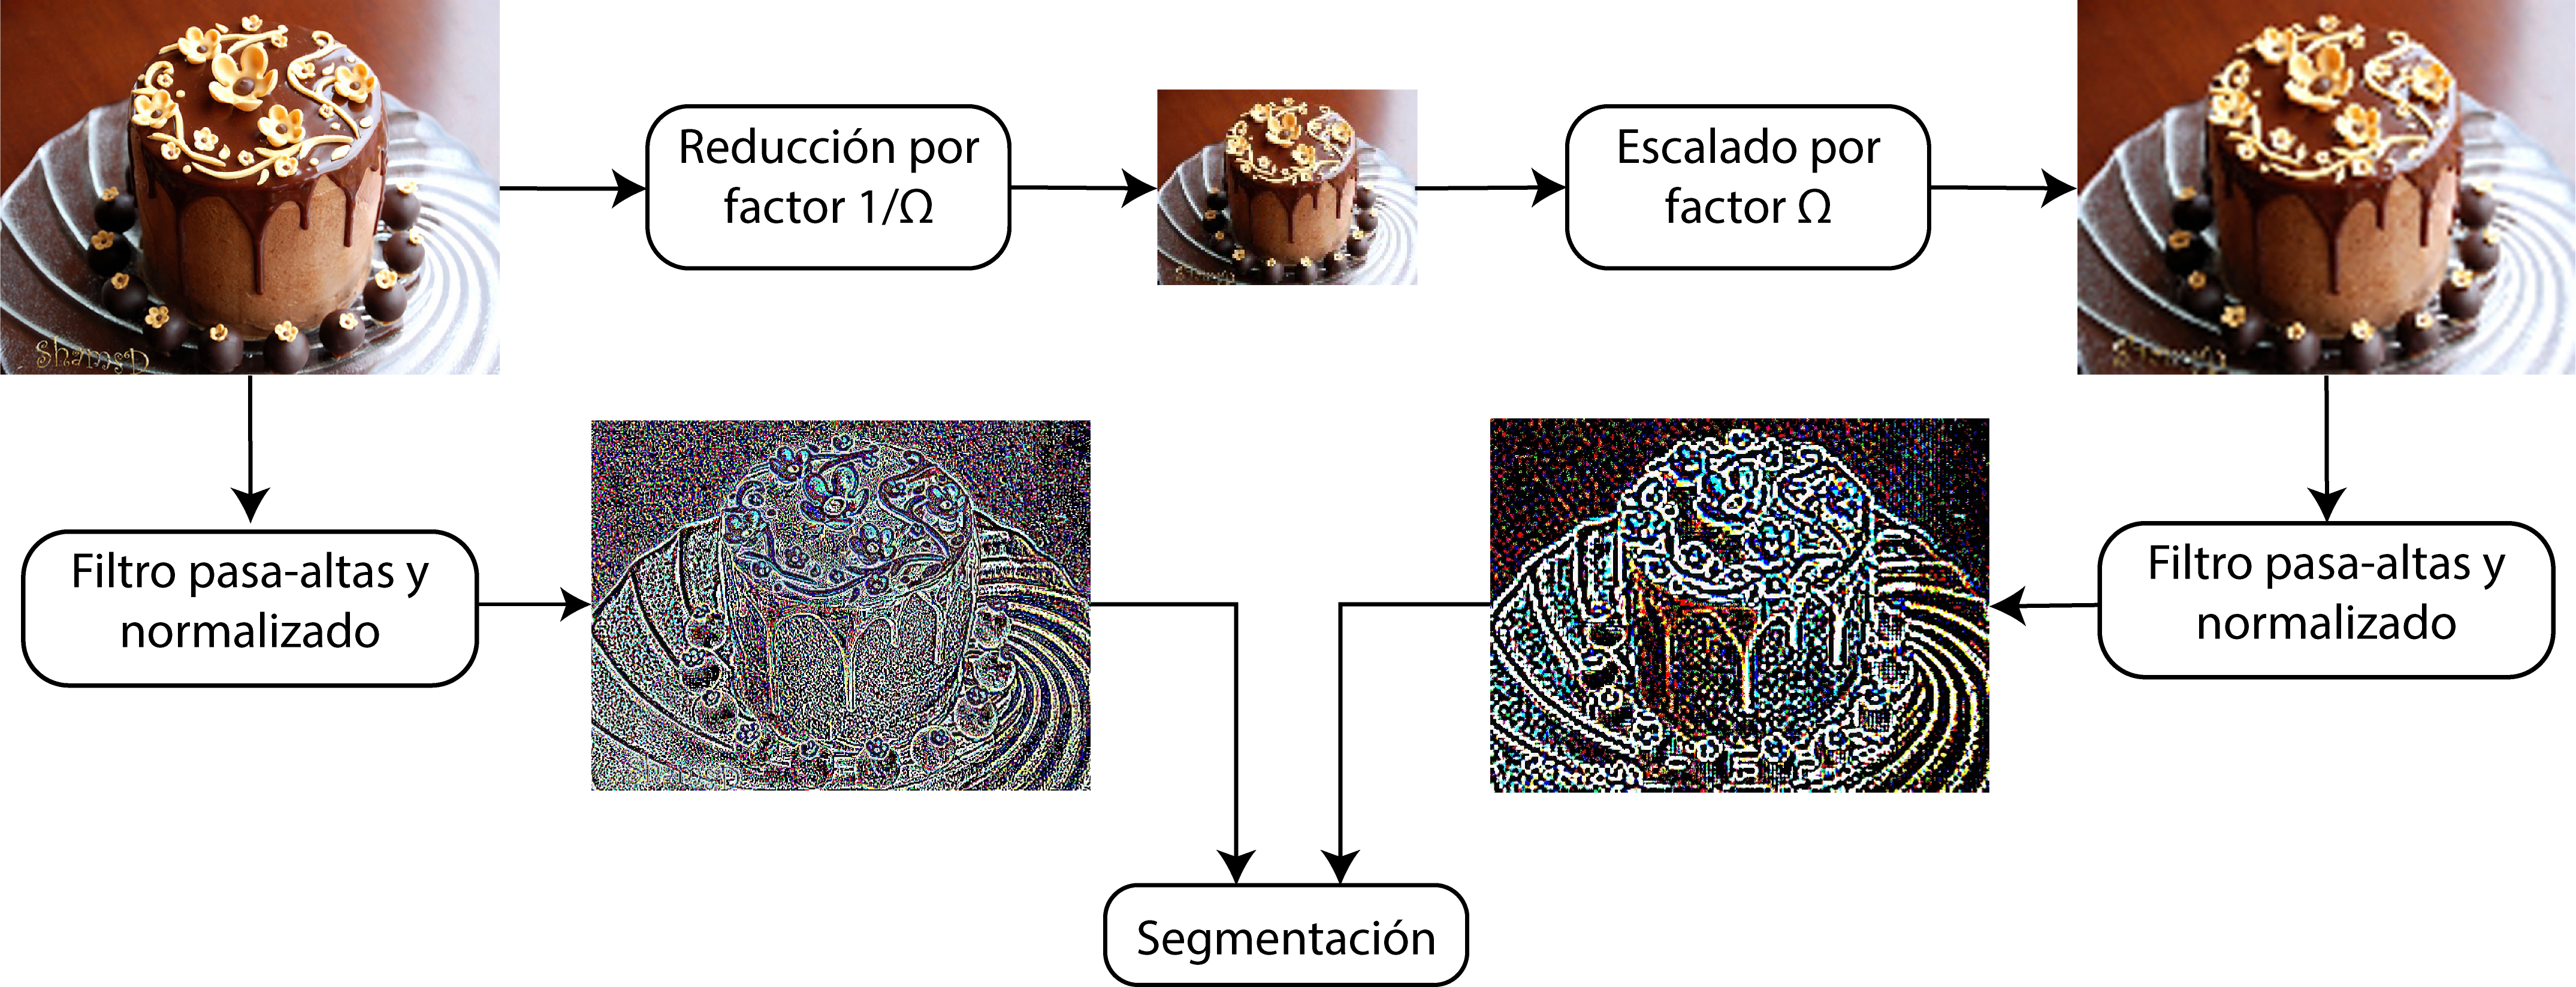
\includegraphics[scale = 0.6]{ fr_prepdic.png }
    \centering
    \caption{Preparación de base de entrenamiento mediante algoritmos de interpolación}
    \label{fig:fr_interpolacion}
\end{figure}

Como se presenta en la Figura \ref{fig:fr_interpolacion}, ambas imágenes 
rquieren ser filtradas (para reducir la cantidad de información innecesaria)
y normalizadas (con el objetivo de generalizar el algoritmo) para realizar el
proceso de segmentación. Para el filtro pasa-altas, se utilizó la función de\
\emph{OpenCV} \emph{GaussianBlur} considerando una desviación estándar $\sigma = 1$
con el fin de restar la imagen desenfocada (frecuencias medias y bajas) a la imagen 
original para dejar sólo las frecuencias altas (detalles) tal como se presenta
en la expresión \eqref{eqn:filtroPH}.

\begin{align}
    \label{eqn:filtroPH}
    \text{img}_f = \text{img} - \text{\emph{cv2.GaussianBlur(img, }(0,0),}\, \sigma)
\end{align}

Respecto al proceso de normalización, se consideró la expresión \eqref{eqn:normalizado}.

\begin{align}
    \label{eqn:normalizado}
    \text{img}_n = \frac{\text{img}_f-\text{min}(\text{img}_f)}{\text{max}(\text{img}_f)-\text{min}(\text{img}_f)}\cdot 255
\end{align}

De esta manera, el \emph{segmentador} puede realizar un barrido bidimensional en cada imagen 
con el objetivo de recolectar los parches en alta y baja resolución con 
dimensiones de $5x5$ y $7x7$ respectivamente.

\begin{figure}[H]
    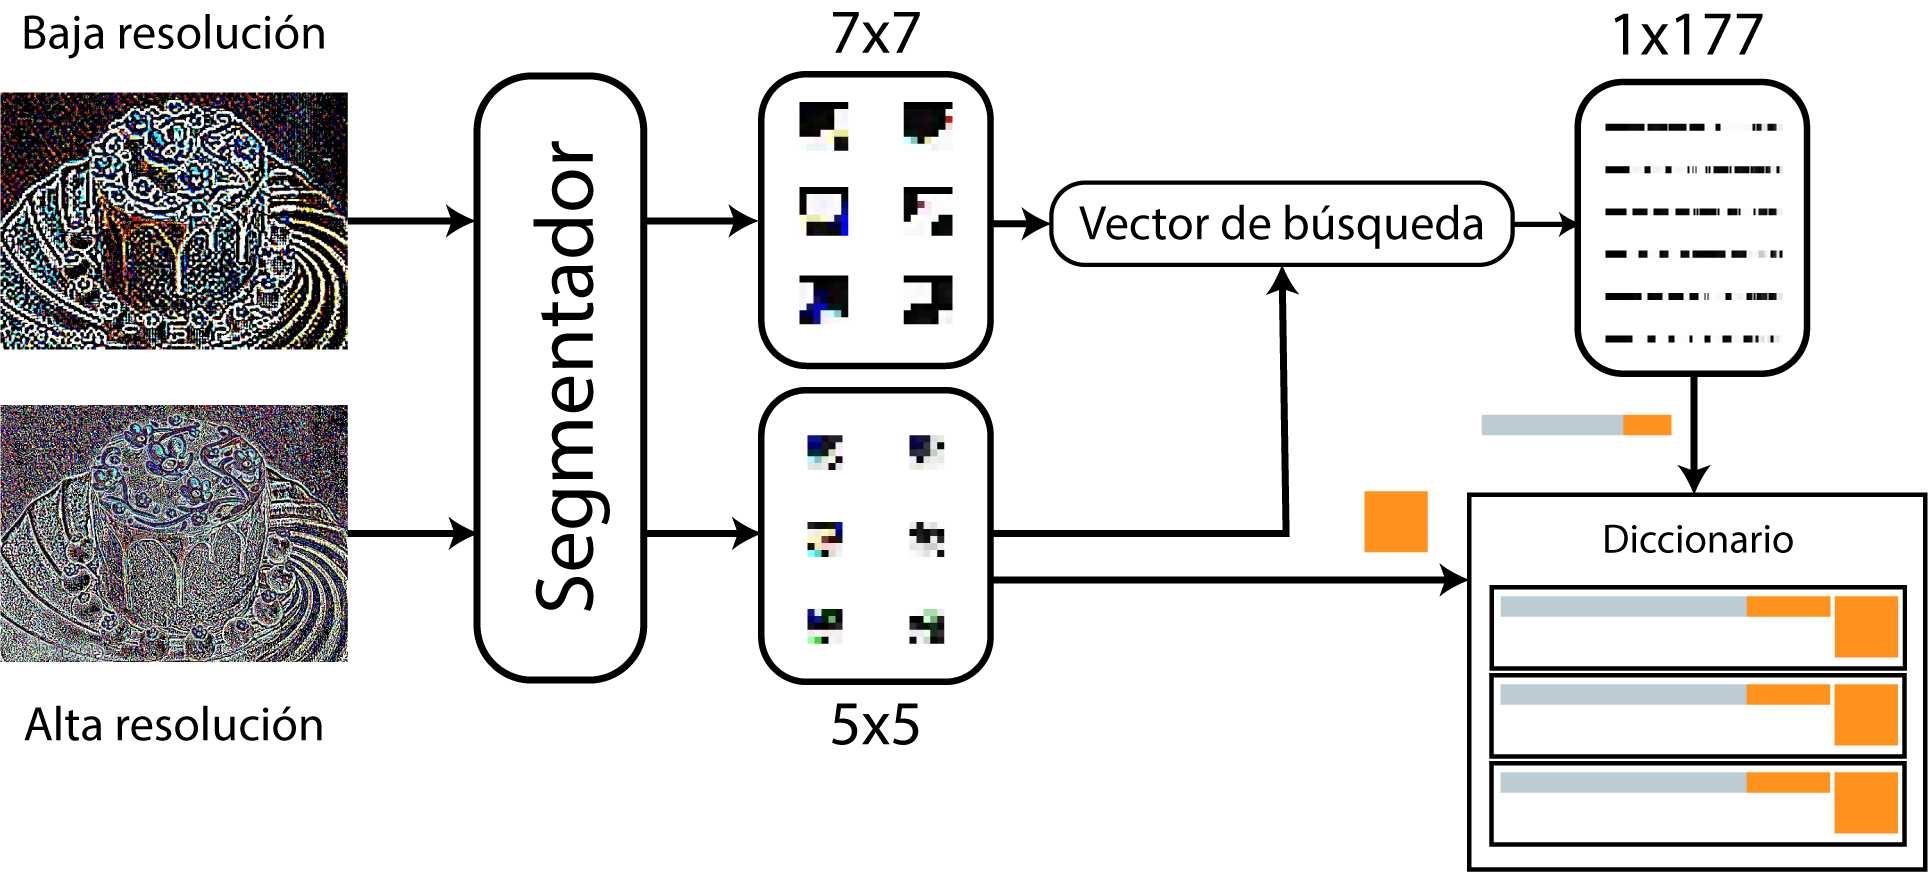
\includegraphics[scale = 1.2]{ fr_segmentado.png }
    \centering
    \caption{ Segmentación y almacenamiento de parches en diccionario }
    \label{fig:fr_segmentador}
\end{figure}

Posteriormente, el parche de baja resolución es reordenado para formar un 
vector fila en $\mathbb{R}^{147}$ para concatenarse con el vector de superposición
(en $\mathbb{R}^{30})$ que considera la primera fila y primera columna del
parche de alta resolución. A dicha concatenación se le nombrará como 
\emph{vector de búsqueda}. En la Figura \ref{fig:fr_segmentador} puede observarse
al conjunto de vectores de búsqueda que serán guardados en el \emph{diccionario}
junto con los parches de alta resolución. 